\chapter{Il sistema chimico}
\vspace{0.5cm}
\label{cha:789}

Una delle proprietà fondamentali degli organismi viventi è l'abilità di sentire e rispondere ai cambiamenti dell'ambiente tramite il movimento. 
Se consideriamo la cellula, in termini generali, come un sistema chimico aperto in una situazione di non-equilibrio, è essenziale avere a disposizione un rifornimento di materiale fresco e di energia per sostenerla. Per fare in modo che questo avvenga, la cellula modifica il suo ambiente esterno metabolizzando risorse di sostentamento e producendo dei prodotti e degli scarti. Per evitare una situazione statica, di equilibrio, il sistema deve trovare in qualche modo nuove risorse ed evitare possibili effetti inibitori dei prodotti di scarto. In questo senso puramente chimico-biologico si crede che l'abilità di movimento giochi un ruolo importante per evitare lo stato di equilibrio nella creazione di sistemi cellulari artificiali. \cite{doi:10.1021/ja0706955}

\section{Chemiotassi e Chemiochinesi}
\label{sec:456}
Le cellule sono in grado di avvertire molecole solubili presenti nell'ambiente esterno ad esse e di percepirne eventuali cambiamenti; sono ad esempio capaci di percepire la formazione di gradienti di concentrazione. 
Una cellula che percepisce delle molecole solubili può muoversi lungo il gradiente di concentrazione creato da queste fino a raggiungere la sorgente oppure allontanarsi da questa nel caso in cui le sostanze rilasciate siano repellenti o tossine.
In generale, la motilità di una cellula può essere di tre tipi:
\begin{enumerate}
\item motilità basale casuale: avviene in assenza di stimoli chimici,
\item Chemiochinesi: corrisponde ad un movimento casuale crescente, in risposta a stimoli chimici,
\item Chemiotassi: migrazione stimolata direzionale verso un gradiente chimico.
\end{enumerate}
La \emph{chemiotassi} può essere di tipo positivo in caso di avvicinamento alla sorgente e di tipo negativo in caso di allontanamento.
	\begin{figure}[h]
	  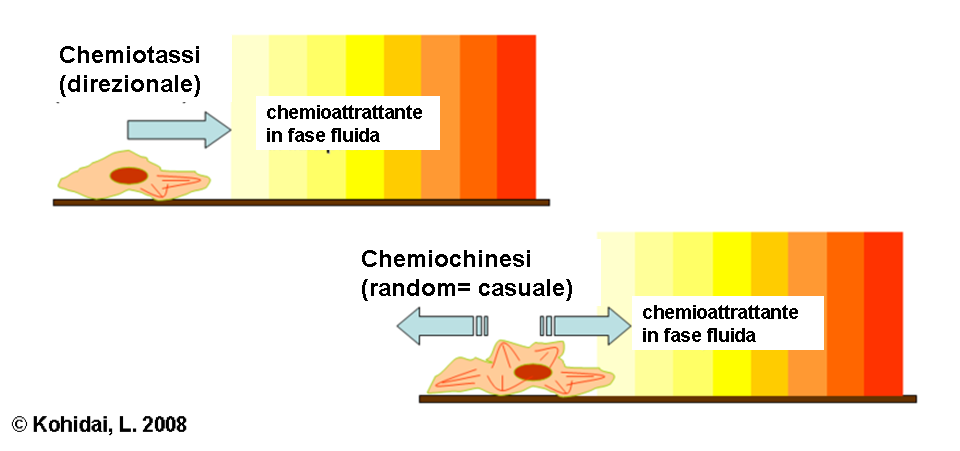
\includegraphics[scale=0.50]{immagini/chemochin.png}
		\centering	
	 \caption{Chemiotassi e chemiochinesi}
	\end{figure}
\pagebreak
\\E' stato qui considerato il movimento chemiotattico positivo promosso da una \emph{droplet} di decanolo in acido decanoico lungo il gradiente di concentrazione creato dall'aggiunta di Cloruro di sodio.
\subsection{L'importanza del movimento}
\label{sec:00456}
Per gli organismi multicellulari la chemiotassi è importante nei processi fisiologici, come il reclutamento di cellule del sistema immunitario nei siti dell'infezione e negli organi dello sviluppo durante l'embriogenesi.\cite{cellMig} Le cellule neuronali e quelle embrionali, invece, migrano durante lo sviluppo. Durante l'angiogenesi, le cellule endoteliali vanno incontro a chemiotassi per formare i vasi sanguigni, mentre le cellule epiteliali e i fibroblasti si muovono con chemiotassi durante la guarigione di una ferita.\cite{move1} Tuttavia, oltre al ruolo in processi ovviamente benefici, la chemiotassi è coinvolta anche in tutti gli stadi cruciali del tumore cellulare, dalla disseminazione alla progressione delle metastasi. Molte cellule cancerogene, nello specifico quelle del tumore al seno, sono note per avere la preferenza nel metastatizzarsi in specifici organi e tessuti. Questa preferenza è correlata alla produzione di chemioattraenti del tessuto e degli organi bersaglio e ad una sovrapproduzione dei recettori di queste sostanze sulla superficie delle cellule cancerose \cite{chemocancer}.
Il movimento spontaneo di \emph{droplet} liquide, particelle solide e gel in condizioni di non-equilibrio, è stato spesso studiato sia a livello teorico che sperimentale. Il movimento di auto-avanzamento di oggetti non biologici può simulare il comportamento chemiotattico o chemiocinetico di cellule viventi.
Come nel caso di organelli mobili e cellule che esibiscono polarità, è necessaria una rottura spontanea della simmetria per scatenare l'auto-movimento di oggetti non-biologici. 
\\Una \emph{droplet} posizionata sulla superficie di un substrato, può muoversi quando la superficie sottostante cambia il proprio motivo in modo asimmetrico creando una differenza nella tensione interfacciale tra il margine anteriore e il margine posteriore della droplet. Inoltre una \emph{droplet} può rompere la simmetria attraverso una reazione chimica accoppiata che avviene all'interfaccia tra la droplet e la soluzione circostante. La reazione chimica produce una rottura della simmetria dovuta all'accumulo e al rilascio di prodotti che inducono la droplet a muoversi attraverso la soluzione acquosa.\cite{selfpropelled}
\\Il motivo del percorso della droplet osservato in questo studio è di tipo rettilineo ed è stato analizzato con un software di analisi visuale. 

\section{Componenti inorganiche}
\label{sec:123}
Questo studio ha esaminato in particolare la dinamica di una \emph{droplet} di decanolo  che si muove chemiotatticamente in una soluzione acquosa di Acido decanoico $(CH_{3}(CH_{2})_8COOH)$ lungo i gradienti di concentrazione formati con l'aggiunta di Cloruro di sodio $(NaCl)$ $3.5M$.\cite{ikea}
\\E' stata analizzata la dipendenza parametrica della risposta chemiotattica della droplet al variare della concentrazione e del pH di Sodio decanoato in rapporto alla forza del gradiente di concentrazione di $NaCl$ $3.5M$. 
Lo spazio multiparametrico utilizzato ha previsto l'esecuzione di ripetizioni di ognuno dei nove esperimenti così composte: 
\begin{table}[h]
\caption{Spazio multiparametrico degli esperimenti}
\begin{center}
\begin{tabular}{l|l|l|l}
\backslashbox{\textbf{molarità}}{\textbf{ph}} & \textbf{11} & \textbf{12} & \textbf{13} \\ \hline
\textbf{20mM} &  &   &   \\ \hline
\textbf{10mM} &    &   &   \\ \hline
\textbf{5mM}  &    &  &  \\ \hline
\end{tabular}
\end{center}
\end{table}

Le soluzioni di acido decanoico in fase acquosa sono state preparate sciogliendo $3,44gr$ di Acido decanoico  in $1L$ di acqua per avere una soluzione $20mM$. Con l'aggiunta di $10mL$ di $NaOH$ si è ottenuta una soluzione con $pH 13$. 
Da questa si sono creati gli \emph{stock}, a $pH13$, da $100mL$ ciascuno per le soluzioni nelle differenti molarità: $5mM$ diluendo $1/4$ del volume con acqua, $10mM$ diluendone $1/2$ e $20mM$ tenendo la soluzione non diluita.
\\Ulteriori $300mL$ della soluzione di partenza sono stati utilizzati per le soluzioni a $pH 12$, il livello desiderato di pH è stato raggiunto con l'aggiunta di $10\mu L$ di $HCl$. Anche di questi si sono create le diluizioni con molarità $5mM$, $10mM$ e $20mM$. 
\\I restanti $300mL$ sono stati utilizzati per le soluzioni a $pH11$ con ulteriore aggiunta di $20\mu L$ di $HCl$; applicando le stesse diluizioni per le stesse molarità.
La soluzione di $NaCl$ utilizzata è stata ottenuta disciogliendo $10,227gr$ di $NaCl$ in acqua per avere la molarità a $3.5M$.
\\Per rendere le droplet di decanolo visibili al software di analisi, si è aggiunto il colorante Oil Red O a $20mL$ di decanolo in piccola quantità, fino al completo scioglimento.  






